
\begin{frame}
%  \frametitle{Манделброт}
  \begin{figure}[t]
    
\includegraphics[height=8.0cm]{Mandel_zoom_00_mandelbrot_set.jpg}
  \end{figure}
\end{frame}
\begin{frame}
%  \frametitle{Манделброт}
  \begin{figure}[t]
    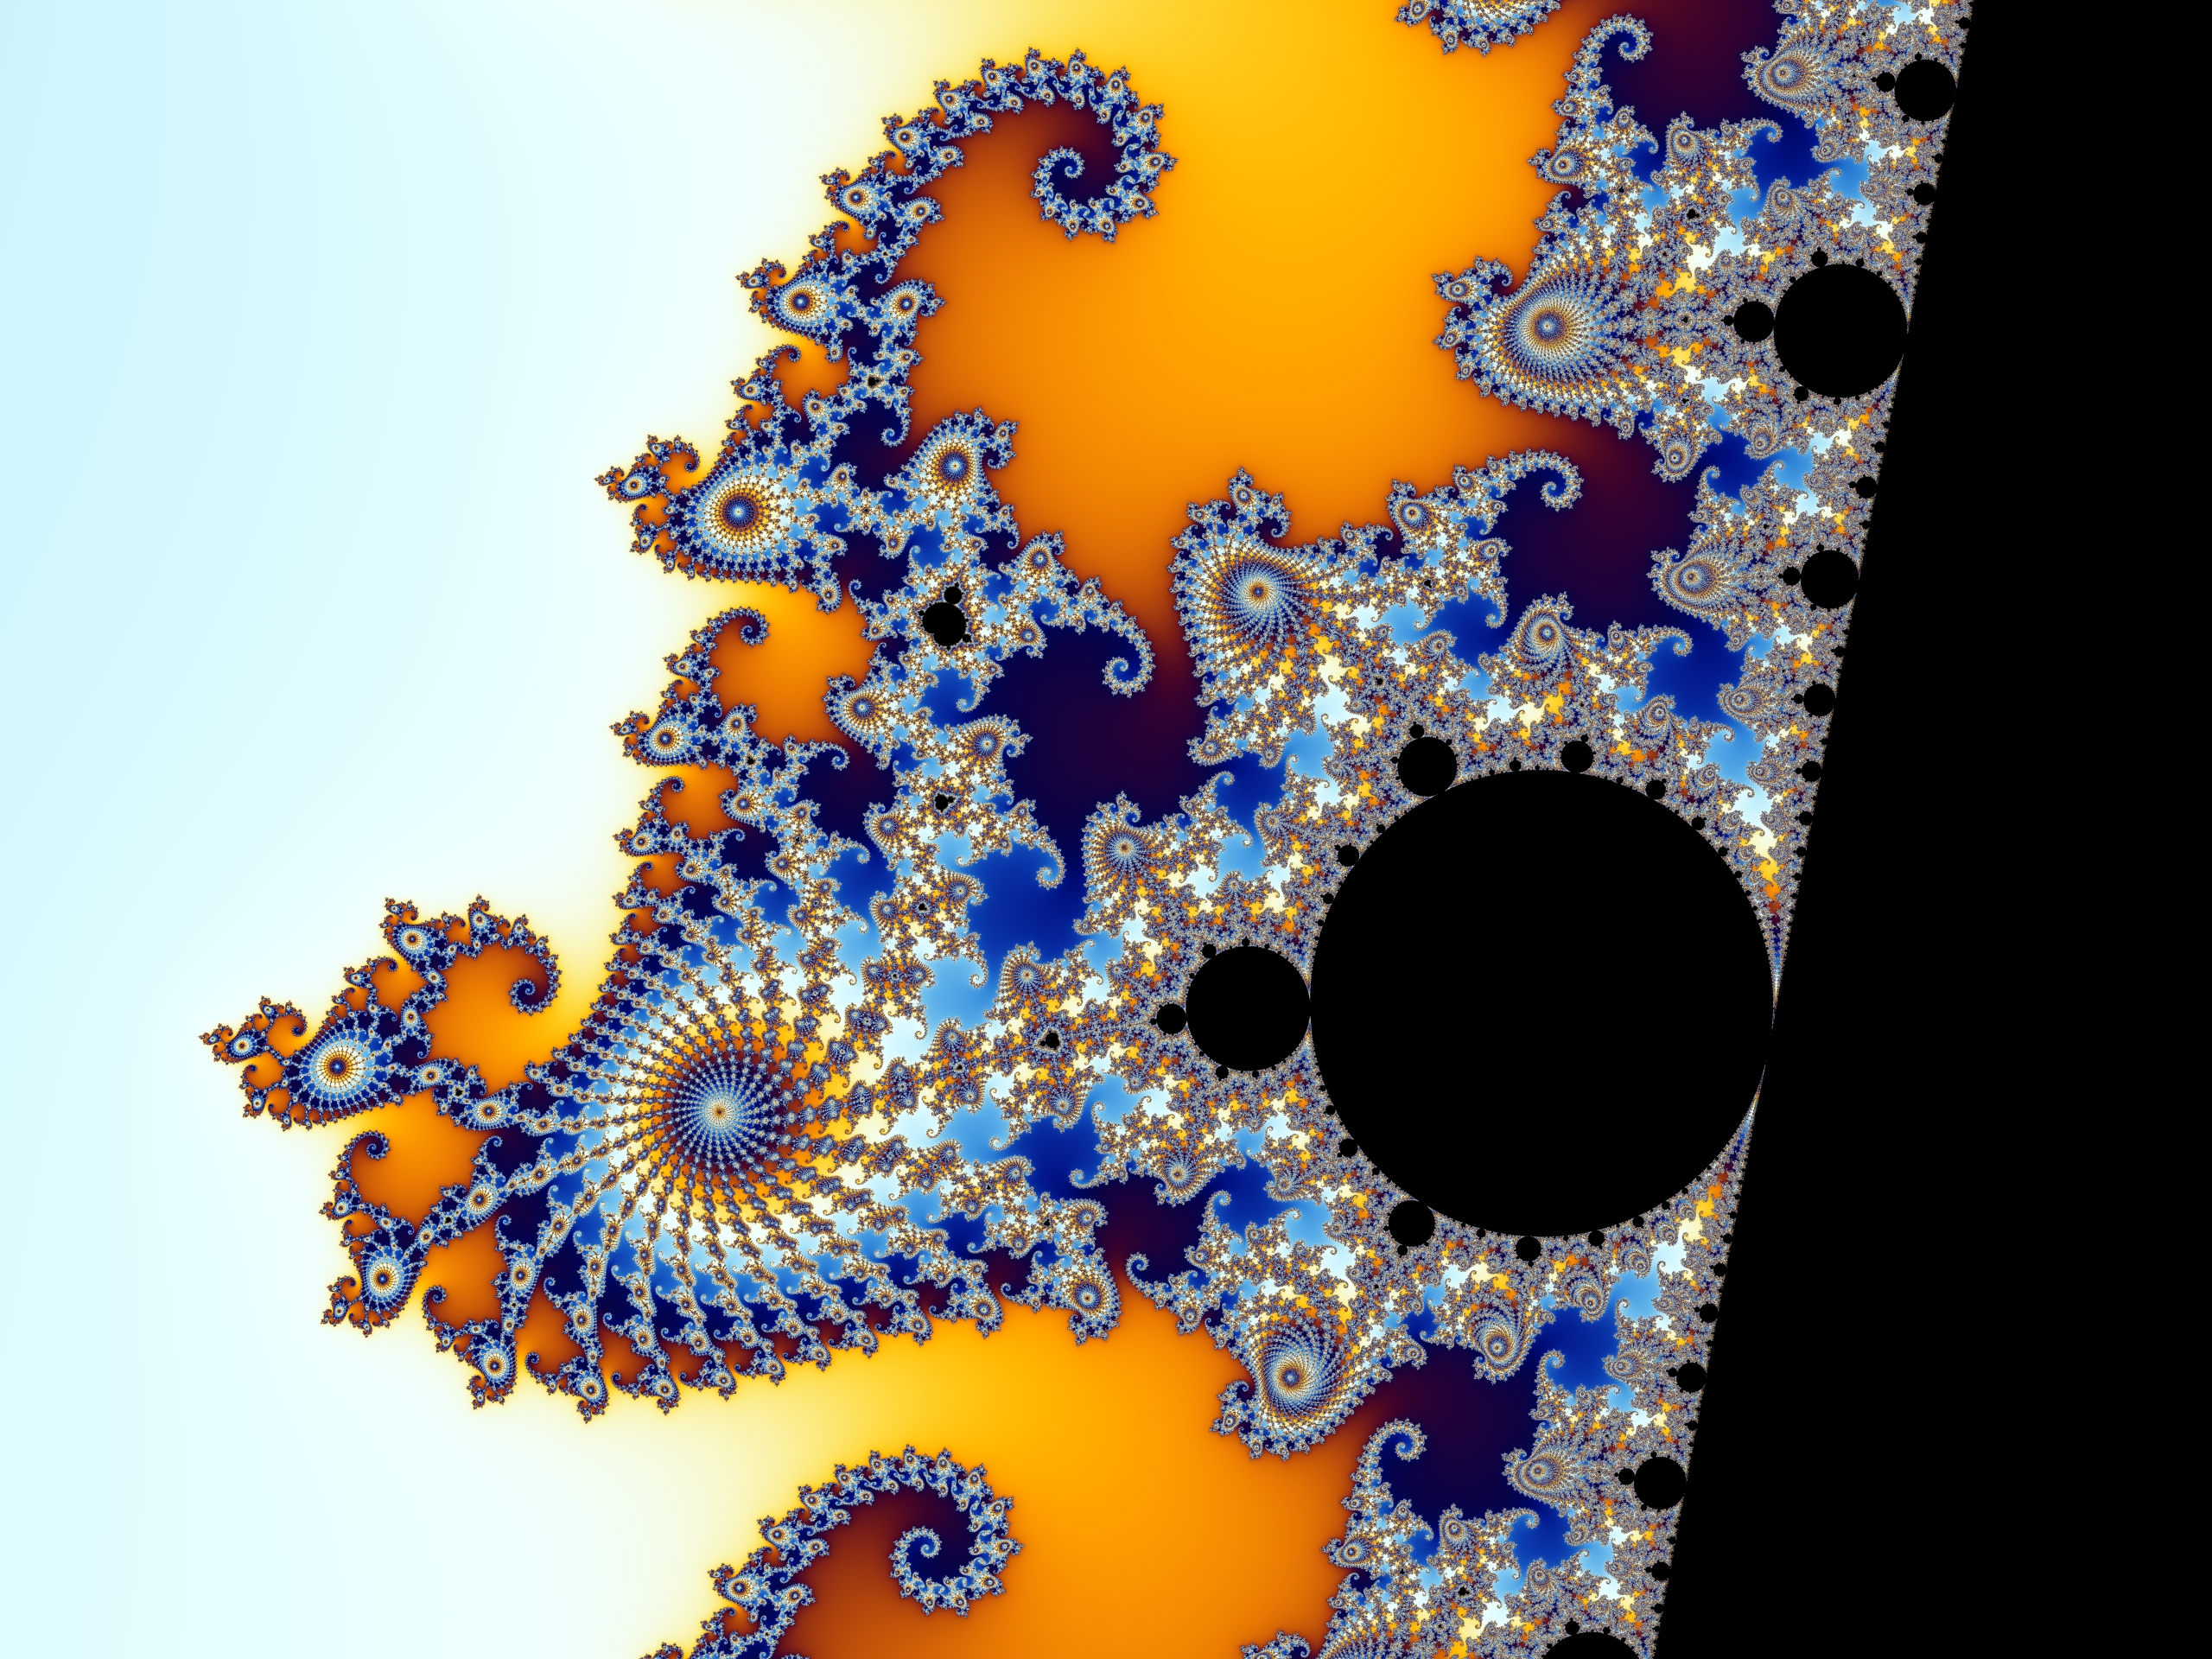
\includegraphics[height=8.0cm]{Mandel_zoom_03_seehorse.jpg}
  \end{figure}
\end{frame}

\begin{frame}[fragile]
  \frametitle{Манделброт - Монте Карло}
  \begin{equation*}
  z_{n+1} = z_n^2 + x + iy, \quad z_0 = 0, \quad x,y \in \mathbb{R} 
  \end{equation*}
  \pause
\begin{lstlisting}
RandomGenerator rng;
int hits = 0;
for (int i = 0; i < nSamples; i++) {
   float x = rng.getUniform(-2.0, 1.0);
   float y = rng.getUniform(-1.0, 1.0);
   int res = inMandelbrot(x,y)? 1 : 0;
   hits += res;
}
float area = hits * 6.0f / nSamples;
\end{lstlisting}
\end{frame}
